\documentclass[hyperref,a4paper,UTF8]{ctexart}
\usepackage{ctex}
\usepackage{datetime}
\usepackage[utf8]{inputenc}
\usepackage{graphicx}
\graphicspath{images}
\usepackage{amsmath}
\usepackage{mhchem}
\usepackage{float}
\usepackage{tabularx}
\usepackage{multirow}
\usepackage[left=2.50cm, right=2.50cm, top=2.50cm, bottom=2.50cm]{geometry}
\usepackage{latexsym,amssymb,amsmath,amsbsy,amsopn,amstext,amsthm,amsxtra,color,bm,calc,ifpdf}
\usepackage{graphicx}
\usepackage{enumerate}
\usepackage{fancyhdr}
\usepackage{listings}
\usepackage{multirow}
\usepackage{makeidx}
\usepackage{xcolor}
\usepackage{fontspec}
\usepackage{subfigure}
\usepackage{hyperref}
\usepackage{pythonhighlight}
\usepackage{float}
\usepackage{mhchem}
\usepackage{amssymb}
\usepackage{booktabs}

\makeatletter
\newcommand{\rmnum}[1]{\romannumeral #1}
\newcommand{\Rmnum}[1]{\expandafter\@slowromancap\romannumeral #1@}
\makeatother

\pagestyle{fancy}
\fancyhead[L]{}
\fancyhead[C]{\fangsong 液体表面张力的测定}
\fancyhead[R]{}
\title{\huge \textbf{液体表面张力的测定}}
\author{尚子翔 522111910161}
\date{\today}

\begin{document}
\maketitle{}
\tableofcontents
\newpage


\section{实验目的}
(1)了解表面张力、表面吸附力的定义及其关系式


(2)掌握最大泡压法测定液体表面张力的原理和技术


(3)测定不同浓度正丁醇水溶液的表面张力,并计算表面吸附量和正丁醇分子的截面积
\section{实验原理}
任何液体都有自动缩小表面积以降低体系能量的趋势,恒温恒压下若液体的表面积增加$\Delta{A}$,则要对体系做的非体积功
\begin{equation}
    W'=\sigma \Delta A
\end{equation}
式中:$\sigma$称为液体的比表面吉布斯函数或表面张力,单位为$J\cdot m^{-2}$或$N\cdot m^{-1}$.$\sigma$是液体自动缩小表面积趋势大小的标志,在恒温、恒压、体系组成和液体表面气氛确定的条件下具有确定值。


当向纯溶剂中加入能降低表面张力的溶质时,根据能量最低原理,溶液表面层中溶质的浓度比内部大;反之,若溶质能使溶液表面张力升高,则溶质在表面层中的浓度比溶液内部小,这种表面浓度与溶液内部浓度不同的现象称为溶液的表面吸附。


恒温恒压下,溶液的表面吸附量与溶液的表面张力及溶质在溶液中的活度之间的关系式为
\begin{equation}
    \Gamma =-\frac{a}{RT} (\frac{\partial \sigma }{\partial a})_{T} 
\end{equation}
式(2)成为吉布斯吸附等温式。溶液浓度较稀时可用浓度代替活度,则式(2)可近似为
\begin{equation}
    \Gamma =-\frac{c}{RT} (\frac{\partial \sigma }{\partial c})_{T} 
\end{equation}
式中$\Gamma$为表面吸附量,单位为$mol\cdot m^{-2}$;$\sigma$为表面张力,单位为$N\cdot m^{-1}$;c为溶液浓度,单位为$mol\cdot m^{-3}$;T为热力学温度,单位为K;R为摩尔气体常量。当$\frac{\partial \sigma }{\partial a}< 0$时,\Gamma>0$成为正吸附;$\frac{\partial \sigma }{\partial a}> 0$时,$\Gamma<0$成为负吸附。


为了获得表面吸附量$\Gamma$,可先测定不同浓度溶液的表面张力,作$\sigma-c$ 曲线图,如图1所示。在曲线上任选一点作切线,则可得该点对应的斜率$(\frac{\mathrm{d} \sigma}{\mathrm{d} c} )_{T}$ ,由式(3)可求得此浓度下溶液的表面吸附量$\Gamma$,再作$\Gamma-c$图,如图2所示,外推可在纵轴上得到溶液表面的饱和吸附量$\Gamma_{\infty}$

\begin{figure}[H]
    \centering
    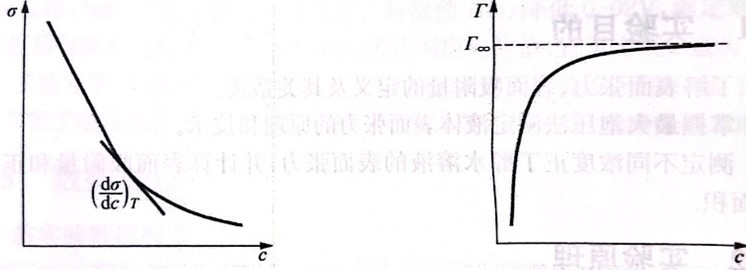
\includegraphics[width=0.5\textwidth,height=0.3\textwidth]{i.jpg}
    \caption{表面张力和表面吸附量与浓度关系图}
    \label{fig:my_label}
\end{figure}



由于溶液表面层吸附可近似为单分子层,因此根据朗缪尔吸附等温式,有
\begin{equation}
    \frac{c}{\Gamma}=\frac{c}{\Gamma _{\infty}}  +\frac{1}{b\Gamma _{\infty}}
\end{equation}
式中:b为吸附常数。作$\frac{c}{\Gamma}-c$图得一直线,直线斜率的倒数即为$\Gamma_{\infty}$。


每个溶质分子在溶液表面所占据的截面积
\begin{equation}
    S_{B}=\frac{1}{\Gamma_{\infty}\cdot L}
\end{equation}
式中:L为阿伏伽德罗常量


液体表面张力的测定方法有最大泡压法、毛细管升高法、滴重法和圆环法等。本实验用最大泡压法测定正丁醇水溶液的表面张力,其装置如图三所示。
\begin{figure}[H]
    \centering
    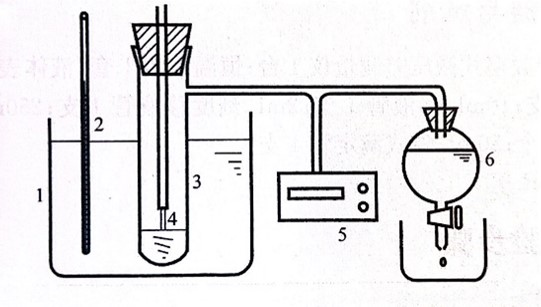
\includegraphics[width=0.5\textwidth]{2.jpg}
    \caption{最大泡压法测定液体表面张力实验装置图}
    \label{fig:my_label}
\end{figure}


由与液面相切的毛细管4鼓出空气泡时,需要高出外部大气压的附加压力以克服气泡的表面张力,此附加压力与表面张力成正比,与气泡的曲率半径成反比,其关系式为
\begin{equation}
    \Delta p=\frac{2\sigma}{r} 
\end{equation}
式中:$\Delta p$为附加压力,$\sigma$为表面张力,r是气泡的曲率半径。如果毛细管半径$R^{'}$很小,则形成的气泡基本上是球形的,当气泡开始形成时,表面几乎是平的,这时曲率半径最大,随着气泡的形成,曲率半径逐渐变小,直到形成半球形,此时曲率半径r与毛细管半径$R^{'}$相等,曲率半径达到最小值,由式(6)知,此时附加压力达到最大。当气泡进一步增大时,r变大,附加压力则变小,直到气泡逸出。由式(6)知,当$r=R^{'}$时最大附加压力
\begin{equation}
    \Delta p_{max}=\frac{2\sigma}{R^{'}}
\end{equation}
有
\begin{equation}
    \sigma=\frac{R^{'}}{2} \Delta p_{max}=K\times \Delta p_{max}
\end{equation}


实际测量时,使毛细管顶端刚与液面接触,则可忽略鼓泡所需克服的静压力,这样就可直接用式(8)计算。


由于直接测量毛细管的半径很不方便,所以实验时用已知表面张力$\sigma_{0}$的液体测定毛细管常数K,则待测液体的表面张力
\begin{equation}
    \sigma=\frac{\Delta p_{max}}{\delta p_{0}} \times \sigma_{0}
\end{equation}
式中:$\sigma$为待测液体的表面张力;$\Delta p_{max}$为待测液体的最大附加压力;$\delta p_{0}$为已知表面张力的液体的最大附加压力。$\Delta p_{max}$与$\delta p_{0}$均需通过实验测定。
\section{仪器与药品}
DP-AW\Rmnum{2}型表面张力实验装置;毛细管1支;10mL移液管1支;2mL刻度移液管1支;洗耳球1个;250mL容量瓶1个;50mL容量瓶9个;50mL碱式滴定管1支


99\%正丁醇(A.R.)

\section{实验步骤}
\subsection{准备工作}
实验前由小到大慢慢开启恒温槽搅拌电动机至适当速率,调节恒温槽温度为25℃\\
(1)配制0.5$mol\cdot dm^{-3}$的正丁醇溶液250mL.按正丁醇的摩尔质量和密度($\rho_{20℃}=809.78kg \cdot m^{-3}$)计算正丁醇的体积。先在250mL容量瓶中装入约一半的去离子水,然后用10mL移液管及2mL刻度移液管吸取所需正丁醇体积放入容量瓶中,加水至刻度,混匀后作为母液,装入50mL碱式滴定管。\\
(2)在50mL容量瓶中用母液配制0.02、0.04、0.06、0.08、0.10、0.12、0.16、0.20和0.24$mol\cdot m^{-3}$浓度的稀溶液备用。
\subsection{数据测定}
\subsubsection{毛细管常数K的测定}
(1)洗净毛细管4和样品管3,用洗耳球吹干毛细管残留液体。


(2)样品管中装适量去离子水,按图3装好,使毛细管的顶端刚好与页面接触


(3)将样品管放在恒温槽1中恒温5min。


(4)达到指定温度后,缓缓打开滴液漏斗6的活塞,使滴液漏斗中的水慢慢滴下,控制滴液速率使毛细管端口鼓出的气泡为单个气泡,且鼓泡速率为5-10s一个气泡。


(5)读取微压差仪上最大压差$\Delta p_{0}$,读取三次取平均值。


\subsubsection{测定不同浓度正丁醇溶液的表面张力}
操作同上,由稀至浓依次测定。注意:更换不同浓度溶液时,需用待测液洗涤毛细管和样品管3次
\section{数据处理与讨论}
实验温度:  25.7℃         


大气压:101.35kpa


%\begin{table}[!ht]
    %%\centering
    %\resizebox{0.8\textwidth}{0.6\textwidth}{}
    %\begin{tabular}{|l|l|l|l|l|l|l|}
    %\hline
       % ~ & ~ & \multicolumn{4}{|c|}{最大压差读数/Pa } & 表面张力${\times}10^{3}/N\cdot m^{-1})$ \\ 
       % \hline
        %~ & ~ &{  1  } &{  2  } &{  3  } & 平均 & ~ \\ 
       % \hline
        %\multirow{10}{*}{正丁醇水溶液浓度/$mol\cdot dm^{-3}$} & 0.00 & ~ & ~ & ~ & ~ & ~ \\ %\cline{2-7}
       % ~ & 0.02 & ~ & ~ & ~ & ~ & ~ \\ \cline{2-7}
        %%~  & 0.04 & ~ & ~ & ~ & ~ & ~ \\ \cline{2-7}
      %  ~  & 0.06 & ~ & ~ & ~ & ~ & ~ \\ \cline{2-7}
       % ~  & 0.08 & ~ & ~ & ~ & ~ & ~ \\ \cline{2-7}
       % ~  & 0.10 & ~ & ~ & ~ & ~ & ~ \\ \cline{2-7}
       % ~  & 0.12 & ~ & ~ & ~ & ~ & ~ \\ \cline{2-7}
       % ~  & 0.16 & ~ & ~ & ~ & ~ & ~ \\ \cline{2-7}
        %~  & 0.20 & ~ & ~ & ~ & ~ & ~ \\ \cline{2-7}
       % ~  & 0.24 & ~ & ~ & ~ & ~ & ~ \\ \hline
      
    %\end{tabular}
    %\caption{各浓度溶液}
%\end{table}


 
\begin{figure}
    \centering
    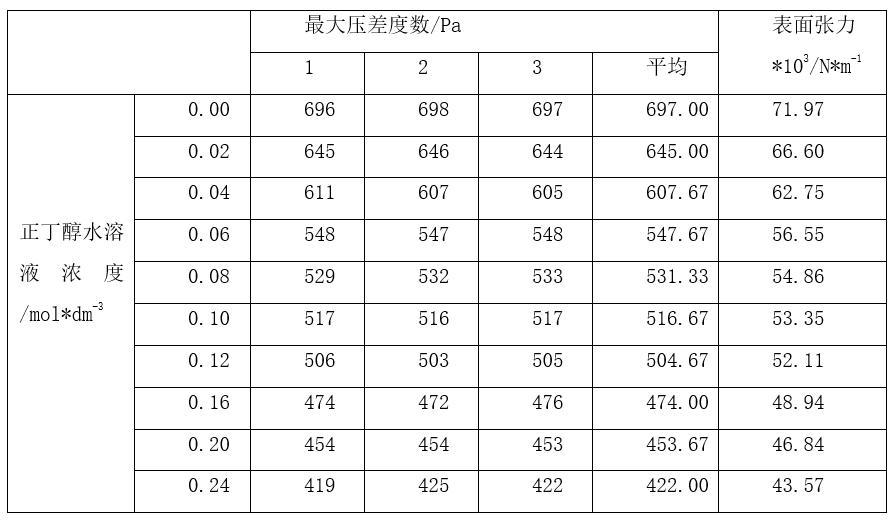
\includegraphics[width=0.75\linewidth]{3.png}
    \caption{原始数据记录}
    \label{fig:enter-label}
\end{figure}
根据$\sigma=\frac{R^{'}}{2} \Delta p_{max}=K\times \Delta p_{max}$ 计算得到毛细管常数$K=1.033 \times 10 ^ {-4}$

作$\sigma$-c图,并根据$\sigma={\sigma _{0}} \times [1-a\cdot lg(1+c/b)]$,得到以下图像
\begin{figure}[H]
    \centering
    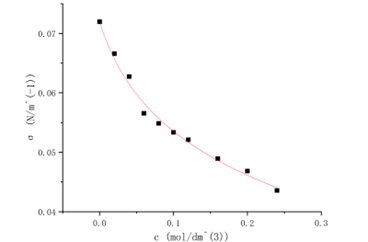
\includegraphics[width=0.8\textwidth,height=0.5\textwidth]{4.png}
    \caption{σ-c图}
    \label{fig:my_label}
\end{figure}
在origin中取20个浓度点并进行微分,然后通过公式$\Gamma =-\frac{c}{RT} (\frac{\partial \sigma }{\partial c})_{T}$ 计算表面吸附量,并作吸附等温Γ-c图.经拟合,发现c=0.24mol/L的点偏离曲线较多,应该在测量时有较大误差,可以视为坏点。所以在拟合时屏蔽该点进行拟合,以减少误差。结果如下:
\begin{figure}[H]
    \centering
    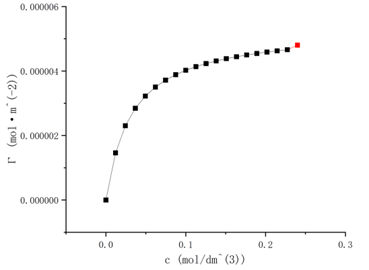
\includegraphics[width=0.8\textwidth,height=0.5\textwidth]{5.png}
    \caption{Γ-c图}
    \label{fig:my_label}
\end{figure}
接着计算$\frac{c}{\gamma}$,并作$\frac{c}{\gamma}$-c曲线,进行线性拟合,得到下图
\begin{figure}[H]
    \centering
    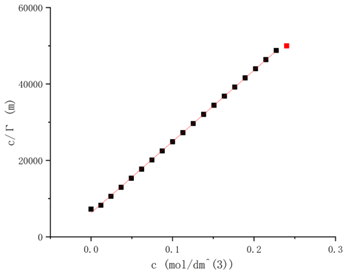
\includegraphics[width=0.8\textwidth,height=0.5\textwidth]{6.png}
    \caption{Γ-c图}
    \label{fig:my_label}
\end{figure}
注:因异常值舍去了第一个点和最后一个点,
根据$\frac{c}{\Gamma}=\frac{c}{\Gamma _{\infty}}  +\frac{1}{b\Gamma _{\infty}}$与拟合所得的方程,计算可得到$\Gamma _{\infty}={5.3582} \times {10^{-3}}mol/m^{2},S_{B}=3.0990 \times 10^{-19}m^{2}$,


根据资料查得正丁醇分子的截面积为$2.4\times 10^{-19}-3.2\times10^{-19}$,因而本次实验相对误差为(-3.16\% ,29.13\%)

可见,实验数据在合理范围之内,但是仍然可能存在误差,可能导致误差的原因有:
\begin{enumerate}
    \item 让毛细管与液面相切这一操作实施的不是很好,毛细管插入液体,产生误差。
    \item 实验要求气泡5-10s出一个,但当正丁醇浓度较高时,气泡放出不再很规律,有时候会几个气泡一起出来,对测定造成影响。
    \item 实验室室温高于25摄氏度(即高于设定温度),以至于开始时水浴温度为25.6摄氏度,而结束时已经有26.4摄氏度了,使得表面张力在实验过程中有所变化,从而造成误差。
    \item 最后一组的数据在拟合时发现有异常偏离,即该点测定误差较大,可能是未将毛细管尖刚好置于溶液表面,或者未控制好气泡冒出速率,以至于有较大误差。
\end{enumerate}


\section{思考题}
(1)为什么保持仪器和试剂的清洁是本实验的关键


因为污染物可能会改名溶液的表面张力,如果存在表面活性剂可能会造成负吸附,导致表面张力升高,如果存在油脂等可能会造成正吸附,导致表面张力降低,实验结果存在误差。


(2)毛细管顶端为何要刚好接触液面?若毛细管插入液体则对实验结果有何影响?


如果毛细管插入液体中,毛细管会有一段水柱,产生额外的压力,这将使测定管中的压力变小,最大压力差变大,从而导致测量结果偏大.


(3)如果气泡出速过快或连续鼓泡,对实验结果有何影响?


当气泡逸出得很快或时,会使液体产生波动,这些波动会影响气泡在液体表面形成和脱离的过程,从而导致最大压力差的读数不准确,从而影响实验最终结果,使结果存在较大误差。
\newpage
\section{附表}
\begin{table}[!ht]
    \centering
    \begin{tabular}{|l|l|l|l|l|l|l|}
    \hline
        c/mol\cdot \textbf{dm}^{-3} & c/mol\cdot \textbf{m}^{-3} & \sigma/10^{-3}{\textbf{N}\cdot \textbf{m}^{-1}}& $(\frac{\mathrm{d} \sigma}{\mathrm{d} c} )_{T}$ & $\Gamma$/$10^{-3}\textbf{mol}\cdot \textbf{m}^{-2}$ & $\Gamma$/\textbf{mol}\cdot \textbf{m}^{-2}$ & $\frac{c}{\Gamma}$ \\ \hline
        0.02 & 20 & 67.05392 & -0.1775 & 0.001408513 & 1.408512678 & 14.19937521 \\ \hline
        0.03157895 & 31.57895 & 64.99864 & -0.16942 & 0.00212273 & 2.122730061 & 14.8765736 \\ \hline
        0.04315789 & 43.15789 & 63.13055 & -0.15459 & 0.002647122 & 2.647122309 & 16.30370076 \\ \hline
        0.05473684 & 54.73684 & 61.41869 & -0.14212 & 0.003086507 & 3.086507437 & 17.73423234 \\ \hline
        0.06631579 & 66.31579 & 59.83929 & -0.1315 & 0.003459992 & 3.459992104 & 19.16645703 \\ \hline
        0.07789474 & 77.89474 & 58.37352 & -0.12238 & 0.003782257 & 3.782256589 & 20.59477938 \\ \hline
        0.08947368 & 89.47368 & 57.00528 & -0.11445 & 0.004062969 & 4.062968958 & 22.02174836 \\ \hline
        0.10105263 & 101.05263 & 55.7231 & -0.10747 & 0.004308909 & 4.308908552 & 23.45202475 \\ \hline
        0.11263158 & 112.63158 & 54.51647 & -0.1013 & 0.004526912 & 4.526911759 & 24.88044521 \\ \hline
        0.12421053 & 124.21053 & 53.37725 & -0.09579 & 0.00472075 & 4.720749931 & 26.31160977 \\ \hline
        0.13578947 & 135.78947 & 52.29808 & -0.09087 & 0.004895748 & 4.8957477 & 27.73620667 \\ \hline
        0.14736842 & 147.36842 & 51.27292 & -0.08642 & 0.005053021 & 5.053020923 & 29.16441912 \\ \hline
        0.15894737 & 158.94737 & 50.29681 & -0.08238 & 0.005195263 & 5.195263041 & 30.59467225 \\ \hline
        0.17052632 & 170.52632 & 49.36515 & -0.07871 & 0.005325418 & 5.325418463 & 32.02120569 \\ \hline
        0.18210526 & 182.10526 & 48.47414 & -0.07535 & 0.005444251 & 5.444251184 & 33.44909224 \\ \hline
        0.19368421 & 193.68421 & 47.6202 & -0.07227 & 0.005553729 & 5.553728929 & 34.87462433 \\ \hline
        0.20526316 & 205.26316 & 46.8005 & -0.06942 & 0.005653638 & 5.653638388 & 36.30638289 \\ \hline
        0.21684211 & 216.84211 & 46.01254 & -0.06679 & 0.005746289 & 5.746289145 & 37.73602485 \\ \hline
        0.22842105 & 228.42105 & 45.2538 & -0.06437 & 0.005833807 & 5.833806768 & 39.15471648 \\ \hline
        0.24 & 240 & 44.52177 & -0.06322 & 0.006020023 & 6.020022861 & 39.86695824 \\ \hline
    \end{tabular}
\end{table}
\end{document}